% \iffalse meta-comment
% Copyright © 2023-2024, RadioNoiseE (Jing Huang)
% Evangelion Japanese Font Metric for LuaTeX
% Current Version: 1.0.5 (c)
% Dev URL: https://github.com/RadioNoiseE/Evangelion-JFM
% \fi
%<*batchfile>
\input docstrip.tex
\keepsilent
\edef\eva{\perCent! TeX Program = LuaLaTeX}
\generate{\usepreamble\eva
          \usepostamble\empty
          \file{Eva-JFM_doc-sc.tex}{\from{\jobname.dtx}{sc}}
          \file{Eva-JFM_doc-jp.tex}{\from{\jobname.dtx}{ja}}
          \file{Eva-JFM_doc-en.tex}{\from{\jobname.dtx}{en}}}
\begingroup\obeyspaces
\Msg{**********************************************}
\Msg{* Now you can run the two generated files:   *}
\Msg{*             Eva-JFM_doc-sc.tex             *}
\Msg{*             Eva-JFM_doc-jp.tex             *}
\Msg{*             Eva-JFM_doc-en.tex             *}
\Msg{* through LuaLaTeX to get the documentation. *}
\Msg{**********************************************}
\endgroup
\endbatchfile
%</batchfile>
%<*sc>
\makeatletter
\def\ltj@stdmcfont{SourceHanSerifSC}
\makeatother
%</sc>
%<*ja>
\makeatletter
\def\ltj@stdyokojfm{eva/{jp,nstd}}
\makeatother
%</ja>
%<sc,ja>\documentclass[twoside]{ltjsarticle}
%<en>\documentclass[twoside]{article}
%<en>\usepackage[margin=1.2in]{geometry}
\usepackage{graphicx}
%<sc>\usepackage[match]{luatexja-fontspec}
%<ja>\usepackage[hiragino-pron, match, deluxe]{luatexja-preset}
%<en>\usepackage{fontspec, luatexja}
%<*en>
\newfontfeature{microtype}{protrusion=default;expansion=default}
\defaultfontfeatures{microtype}
\adjustspacing=2
\protrudechars=2
%</en>
\setmainfont{Linux Libertine O}
%<sc>\setmainjfont{Source Han Serif SC}[Language = Chinese Simplified, YokoFeatures = {JFM = eva/{smpl, nstd, hgp}}]
\setsansfont{Linux Biolinum O}
\setmonofont[Scale = MatchLowercase, FakeStretch = 1.137121]{Iosevka Slab}
%<*sc,ja>
\usepackage{luatexja-adjust}
\ltjenableadjust[priority = true]
%</sc,ja>
\usepackage{listings}
\lstset{
    basicstyle = \ttfamily\small,
    breaklines = true,
    columns = fullflexible,
    keepspaces = true,
    numbers = left,
    numberstyle = \tiny,
    stepnumber = 1,
    gobble = 4,
    numbersep = 6pt,
    escapechar = §
}
\usepackage{hyperref}
\hypersetup{
    hidelinks,
    pdftitle = {Evangelion-JFM},
%<sc,ja>    pdfauthor = {黄京},
%<en>    pdfauthor = {Jing Huang},
    pdfsubject = {TeX},
    pdfkeywords = {Japanese Font Metric},
    pdfstartview = FitV
}
\long\def\feature#1#2#3{{\vskip8pt\vbox{\normalsize\parindent=\zw\hangindent=2\zw\rightskip=2\zw\texttt{#1 --> ({\itshape #2\/})}\\\indent#3\par}}}
\def\meta#1{{\normalfont\rmfamily\itshape$\langle$#1\/$\rangle$}}
%<sc,ja>\def\空{\quad}
%<sc,ja>\def\段{\par}
\def\LuaTeX{Lua\kern-.2ex\TeX}
\def\pTeX{p\kern-.2ex\TeX}
\def\pdfTeX{pdf\TeX}
\title{\sffamily\bfseries Evangelion Japanese Font Metric for \LuaTeX}
\author{\large \url{https://github.com/RadioNoiseE/Evangelion-JFM}\\\url{https://www.ctan.org/pkg/evangelion-jfm}}
%<sc>\date{西历2023年\quad{}黄京}
%<ja>\date{\西暦\today\quad{}黄京}
%<en>\date{2023, Jing Huang (黄京)}
\begin{document}
%<sc,ja>\lstset{doubleletterspace = true}
%<sc>\parindent=2\zw\parskip=2pt
%<en>\parindent=12pt\parskip=2pt
\maketitle

\begin{abstract}
%<sc>    本文档将介绍名为Evangelion Japanese Font Metric(下简称为``\textsf{Eva-JFM}'')的JFM文件。其适用于简体中文(以下简称为「简中」)、繁体中文(以下简称为「繁中」)及日文字体的横直排。旨在提供一个充分利用\LuaTeX-ja的\texttt{priority}特性,基于标准\cite{jlreq}的同时,支持一些罕用特性的JFM文件。文档使用中文、日文及西文撰写。
%<ja>    本ドキュメントは、高品質な中国語および日本語のドキュメントを組版するための日本語フォントメトリック「Evangelion Japanese Font Metric(以下「\textsf{Eva-JFM}」とする)」を紹介するものです。このメトリックは、縦書きと横書きの両方のテキストに対して、従来の中国語、簡体字中国語、および日本語のフォントとともに使用できます。これは、\LuaTeX-ja で提供される優先機能を最大限に活用するフォントメトリックを提供し、標準\cite{jlreq}に基づき、一部の高度な(すなわち、めったに使用されない)機能をサポートすることを目的としています。\段
%<ja>    本ドキュメントは、完全なものではありません。文法的な(および文脈的な)エラーが多数含まれている可能性があります。
%<en>    This documentation is going to introduce Evangelion Japanese Font Metric (hereinafter referred to as ``\textsf{Eva-JFM}''), a Japanese Font Metric for typesetting high quality Chinese and Japanese documents. It can be used with Traditional Chinese, Simplified Chinese and Japanese fonts for both vertically and horizontally typesetted texts. It aims to provide a font metric which makes full use of the \texttt{priority} feature (provided by \textsf{\LuaTeX-ja}), bases on the standard~\cite{jlreq}, and supports some advanced (a.k.a., rarely-used) features. The documentation is now written in Chinese, Japanese and English.\par
%<en>    This documentation is far from complete. It may have many grammatical (and contextual) errors.
\end{abstract}

\tableofcontents

%<sc>\section{背景及略介}
%<ja>\section{背景情報と簡単な紹介}
%<en>\section{Background Information and a Rough Introduction}
%<sc>\TeX{}是高德纳教授于20世纪末开发的强大排版引擎,能够完全满足西文排版的需求。然因时代局限性\footnote{如没有事实上的统一字符编码等。}以及客观原因\footnote{如中日字符集较大,以及书写方式的不同(纵书、横书),标点等。}对中日排版支持十分有限。为达成中日排版需求,在宏扩展(如\textsf{CJK}等)之外出现了引擎扩展。影响力较大的是\pTeX{}系列。\段
%<ja>{\TeX}は「美しい本の制作」を目的とした強力な組版システムであり、英語ベースのテキストの組版には完全に対応しています。しかし、CJテキストのサポートは限られています\footnote{おそらく普遍的に認められたCJ文字セット標準やエンコーディングシステムが存在しなかったためかもしれません。}。{\TeX}でCJテキストを扱うために、マクロ拡張(\textsf{CJK}など)やエンジン拡張が開発されました。最も影響力のあるものの1つが{\pTeX}(シリーズ)です。\段
%<en>{\TeX} is a powerful typesetting system ``intended for the creation of beautiful books'', it has full support for typesetting English based texts. However, its support for CJ text is limited\footnote{Maybe because there was no universally recognized or accepted CJ character set standard as well as an encoding system.}. For handling CJ texts in {\TeX}, both macro extensions (i.e., \textsf{CJK}) and engine extensions were developed. One of the most influential one is (the) {\pTeX} (series).\par
%<sc>\pTeX{}系列采用虚拟字体的理念,使用\texttt{TFM/VF}映射TrueType或OpenType字体完成排版。其不支持宏配置字体,也不支持直接生成PDF格式文件。但可以满足日本的传统横纵排版需求(工业标准)。\段
%<ja>{\pTeX}は仮想フォント方式を使用し、TrueTypeやOpenTypeフォントを\texttt{TFM/VF}ファイルを使ってマッピングします。マクロを介したフォント設定には対応せず、PDF形式の出力にも対応していません。その利点は、伝統的な日本語のタイポグラフィレイアウト要件を扱うための証明済みの能力にあります。\段
%<en>{\pTeX} uses a virtual font scheme, by mapping TrueType or OpenType fonts using \texttt{TFM/VF} files. It doesn't support font configuration through macros, and has no support for PDF format output. Its advantage is the proven ability for dealing with traditional Japanese typographic layout requirements.\par
%<sc>\pdfTeX{}则是当时另一个\TeX{}的引擎扩展,支持不经DVI格式直接输出PDF格式的文件。然对Unicode(字符编码)及TrueType、OpenType(「现代」矢量字体格式)的支持繁琐或有限。\段
%<ja>{\pdfTeX}は、PDFファイルを直接出力できる{\TeX}エンジンの拡張です(その名の通り)。ただし、Unicodeや現代のフォント形式(TrueTypeやOpenTypeベクターフォント形式)に対するサポートは限定的です。\段
%<en>{\pdfTeX} is a {\TeX} engine extension which can directly output PDF files (just as its name). But it has limited support to Unicode as well as modern font formats (TrueType and OpenType vector font formats).\par
%<sc>\LuaTeX{}便是基于\pdfTeX{}的引擎扩展,在原生支持Unicode下提供Lua语言扩展(使能够使用\textsf{fontloader}等模块)支持现代字体。宏配置字体特性由\textsf{luaotfload}宏集提供。它也支持直接生成PDF文件。\段
%<ja>{\LuaTeX}は{\pdfTeX}をベースにしています。Luaの組み込みにより、読み込みモジュールを使用してUnicodeをサポートし、\textsf{fontloader}を使用して現代のフォントをサポートすることができます。マクロベースのフォント設定機能は\textsf{luaotfload}によって提供されます。\段
%<en>{\LuaTeX} is based on {\pdfTeX}. The inclusion of Lua enables it to support Unicode with the \textsf{reader} module, and modern fonts by using \textsf{fontloader}. Its macro based font setup feature is provided by \textsf{luaotfload}.\par
%<sc>\LuaTeX{}-ja可看作是对两者的合并。这是一个由日本开发者北川弘典首倡的\LuaTeX{}下的日文支持项目,即将\pTeX{}(大部分)移植到\LuaTeX{}下。由于\LuaTeX{}支持宏配置字体,故不需要\texttt{VF}文件为字体提供映射,但为标点挤压等需求保留并扩展\footnote{如优先挤压(\texttt{priority})特性,及一些特殊字符(如\texttt{parbdd}、\texttt{glue})等。}了JFM文件。\段
%<ja>\LuaTeX-jaは{\pTeX}と{\LuaTeX}の移植版と見なすことができます。{\LuaTeX}を使用する場合、マクロによるフォント設定がサポートされるため、{\pTeX}の\texttt{VF}ファイルを保持する必要はありません。しかし、一部の高度な機能(「優先度」機能や仮想的な文字など)は、いわゆるJFMファイルで残され、拡張されました。\段
%<en>\LuaTeX-ja can be seen as a porting of {\pTeX} and {\LuaTeX}. It's a macro package for typesetting high quality Japanese documents when using {\LuaTeX}. {\LuaTeX} supports font configuring by macros, therefore there's no need to keep {\pTeX}'s \texttt{VF} file. But for advanced features it left and extended\footnote{The \texttt{priority} feature and some imaginary characters as well.} the so-called JFM file.\par
%<sc>本项目就是一个JFM文件。使用\LuaTeX{}的\texttt{callback},将简中、繁中、日文及横纵方向、行间标点、悬挂标点、压缩字体等特性集中于\texttt{jfm-eva.lua}单个文件中。用户可按需调用特性来完成高质量的中日排版。
%<ja>このドキュメントでは、高度なJFMファイルである\textsf{Eva-JFM}を説明します。{\LuaTeX}のコールバックを使用して、\texttt{Eva-JFM.lua}にCJテキスト組版に必要な機能を埋め込みます(おそらく)。現在サポートされている機能は、「繁体字中国語」、「簡体字中国語」、「日本語」、「縦組」、「ぶら下げ」、「行間句読点」、「全角歐文」、「半角歐文」、「非標準」。\段
%<en>This document describes \textsf{Eva-JFM}, an advanced JFM file. By using {\LuaTeX}'s callback, it embeds features (maybe) needed in CJ text typesetting in \texttt{Eva-JFM.lua}. The features supported now are ``Traditional Chinese'', ``Simplified Chinese'', ``Japanese'', ``Vertical Typesetting'', ``Linegap Punctuations'', ``Hanging Punctuations'', ``Extended Font'', and ``Non Standard''.

%<sc>\section{安裝及本地配置}
%<ja>\section{インストールとローカル設定}
%<en>\section{Installation and Local Configurations}
%<sc>本项目将源文件托管于GitHub平台,且已上传至Comprehensive \TeX{} Archive Net(CTAN)。用户可使用
%<ja>ソースファイルはGithubにホストされ、CTANにもアップロードされています。ユーザーは単純に
%<en>The sourcefiles are hosted on Github while it's also uploaded to CTAN. Users can simply use
\begin{lstlisting}
    tlmgr install evangelion-jfm
\end{lstlisting}
%<sc>或使用其他包管理器安装。用户也可使用
%<ja>(または他のパッケージマネージャーを使用することもできます)を使用してインストールできます。ただし、CTANブランチが常に更新されているわけではないことに注意してください。 開発者はまた
%<en>(or maybe using other package managers) to install. (But note that the CTAN branch is not always updated.) Developers can also use
\begin{lstlisting}
    mkdir Evangelion-JFM [&&] cd Evangelion-JFM
    git clone https://github.com/RadioNoiseE/Evangelion-JFM
\end{lstlisting}
%<sc>获取源文件,再将其放置在本地的\texttt{TEXMF}路径中,如
%<ja>を使用して最新バージョンを抽出し、それを\texttt{TEXMF}ディレクトリに移動することもできます。たとえば
%<en>to extract the latest version, then move it to the \texttt{TEXMF} directory, for instance
\begin{lstlisting}
    ~/Library/texlive/2023/texmf-dist/tex/luatex/eva-jfm
\end{lstlisting}
%<sc>等。最后运行
%<ja>あなたの{\TeX}配布が\texttt{Ls-R}データベースを更新するためにを
%<en>If your {\TeX} distribution requires
\begin{lstlisting}
    mktexlsr
\end{lstlisting}
%<sc>更新本地\TeX{}的\texttt{Ls-R}文件即可。\段
%<ja>を必要とする場合は、それを実行してください。\段
%<en>to update the \texttt{Ls-R} database, make it so.\par
%<sc>本文件一般情况下无需用户进行本地配置,但若有特殊需求可见第\ref{sec:config}节。
%<ja>\textsf{Eva-JFM}はほとんどの場合、ローカル設定を必要としませんが、特別な要件がある場合は、セクション\ref{sec:config}を参照してください。
%<en>\textsf{Eva-JFM} doesn't require any local configuration in most cases, but if you have some special requirements, have a look at section \ref{sec:config}.

%<sc>\section{使用}
%<ja>\section{使用}
%<en>\section{Using}
%<sc>以下是在\LaTeX{}下使用繁中字体进行直排的示例
%<en>The above is an example of typesetting vertical text using Traditional Chinese fonts
\begin{lstlisting}
    \usepackage{luatexja-fontspec, luatexja-adjust}
    \setmainjfont{Source Han Serif TC}[Language = Chinese Traditional, TateFeatures = {JFM = eva/{vert, trad, nstd}}]
    \ltjenableadjust[priority = true]
\end{lstlisting}
%<sc>(注意需要调用支持直书的文档类或使用\texttt{\string\tate}命令)。\LuaTeX-ja的JFM语法为:
%<ja>\indent 上記は、縦書きの伝統的な中国語フォントを使用して縦書きのテキストを組版する例です。注意が必要ですが、縦書きのテキストをサポートするドキュメントクラスを読み込むか、\texttt{\string\tate}コマンドを使用する必要があります。\LuaTeX-jaのJFM構文は、次のようになります
%<en>(and be aware that you need to load a document class which supports vertical typesetting or use the \texttt{\string\tate} command. \LuaTeX-ja's JFM syntax is the above
\begin{lstlisting}
    jfm = §\meta{JFM name}§/{§\meta{JFM features}§}
\end{lstlisting}
%<sc>而一般情况使用\texttt{\string\setmainjfont}时则为:
%<ja>{\LaTeX}の場合、\texttt{\string\setmainjfont}を使用する場合、最も一般的なケースは、以下のようになります
%<en>while under {\LaTeX} the most common case while using \texttt{\string\setmainjfont} is most likely
\begin{lstlisting}
    \setmainjfont{§\meta{font name}§}[Language = §\meta{language name}§, §\meta{dir}§ = {JFM = §\meta{JFM name}§/{§\meta{JFM features}§}}]
\end{lstlisting}
%<sc>其中,\meta{font name}自然为需要的字体名称。\meta{language name}在使用日文字体时可忽略,而使用简中、繁中字体时为必填\footnote{简中填\texttt{Chinese Simplified},繁中填\texttt{Chinese Traditional}即可。},因\LuaTeX-ja会默认将其覆盖为\texttt{Japanese}选项,而这会带来灾难性的后果\footnote{比如错误的标点位置:日文为冒号及分号中置、其余偏靠,简中是全部偏靠,而繁中则是统统中置。}。\meta{dir}选填\texttt{TateFeatures}(直书)或\texttt{YokoFeatures}(横书)。其后的\meta{JFM name}为调用JFM的文件名\footnote{\LuaTeX-ja会依\texttt{jfm-\meta{JFM name}.lua}的格式来查找该文件。}。最后的\meta{JFM features}选项为选择使用的JFM特性,详细请看第\ref{sec:feat}章。\段
%<ja>オプションの\meta{font name}は、文書のメインフォントとして指定したいフォントの名前です。日本語のフォントを使用する場合、\meta{language name}は自動的に\LuaTeX-jaによって補完されるため、無視してください。この場合、伝統的な中国語フォントには\texttt{Chinese Traditional}、簡体字中国語フォントには\texttt{Chinese Simplified}を指定する必要があります(これを指定しないと、出力が間違った細部、例えば句読点の形状と方向が変わってしまう可能性があります)。\meta{dir}は、縦書きの場合は\texttt{TateFeatures}、横書きの場合は\texttt{YokoFeatures}に設定します。JFMの名前は\meta{JFM features}オプションで指定します\footnote{\LuaTeX-jaは\texttt{jfm-\meta{JFM name}.lua}という方法でJFMファイルを検索します。}。最後に、\meta{JFM features}キーにJFMの特徴を入力してください。これらは、セクション\ref{sec:feat}で説明されています。
%<en>Option \meta{font name} is the font (that you'd like to specify as the main font for your document)'s name. When using Japanese fonts, simply ignore the \meta{language name} since \LuaTeX-ja will automatically fill it for you. In this case, filling \texttt{Chinese} \texttt{Traditional} for Traditional Chinese fonts and \texttt{Chinese} \texttt{Simplified} for Simplified Chinese fonts is necessary\footnote{Without this, your output may result in wrong details, for instance wrong punctuation shape \& direction.}. \meta{dir} should be \texttt{TateFeatures} when typeset vertically and \texttt{YokoFeatures} for typesetting horizontally accordingly. The JFM's name is specified by the \meta{JFM name} option\footnote{\LuaTeX-ja searchs for a JFM file following the method \texttt{jfm-\meta{JFM name}.lua}.}. Finally, for the \meta{JFM features} key, fill in the JFM features. They are described in section \ref{sec:feat}.\par
%<sc>对于进阶用户,也推荐用
%<ja>上級ユーザーの場合、以下を使用することをお勧めします
%<en>For advanced users, it's also recommanded to use the following
\begin{lstlisting}
    \def\ltj@stdyokojfm{eva/{§\meta{JFM features}§}}
\end{lstlisting}
%<sc>或配合NFSS来使用。\段
%<ja>またはNFSSを使用することもできます。\段
%<en>or with the NFSS.\par
%<sc>其他情况下设置JFM及其更多信息请看\LuaTeX-ja文档\cite{luatexja-doc}。
%<ja>他の場合でJFMを設定するには、\LuaTeX-jaのドキュメント\cite{luatexja-doc}を参照してください。
%<en>To set up JFM in other cases, please refer to the \LuaTeX-ja document~\cite{luatexja-doc}.

%<sc>\section{支持特性}
%<ja>\section{サポートされる機能}
%<en>\section{Supported Features}
\label{sec:feat}
%<sc>本章节将介绍\textsf{Eva-JFM}的所有特性,分别为:语言特性、方向特性、扩展特性、西文特性及私有特性。
%<ja>このセクションでは、\texttt{Eva-JFM}に組み込まれたすべての機能を概観します。それらは5つのグループに分けられ、それぞれ次の5つのサブセクションで説明されています。
%<en>This section is going to give you a glance at all the features embedded in \textsf{Eva-JFM}. They are divided into 5 groups, and are described in the next 5 subsections respectively.

%<sc>\subsection{語言特性}
%<ja>\subsection{言語機能}
%<en>\subsection{Language Features}
%<sc>本区特性必填且只可填一个。不然则会报错。\段
%<ja>このセクションから1つの機能を指定する必要があります。そうしない場合、{\TeX}はエラーを出します。\段
%<en>You should specify one and only one feature from this section, or your {\TeX} is going to complain about it.\par
\feature{jp}{JaPanese}{%
%<sc>    日本语特性。当使用日文字体时需调用该特性。其与简中、繁中区别在于问号及感叹号后插入的伸缩胶量。影响特性\texttt{lgp},且对内部分组有影响。
%<ja>    日本語フォント機能。日本語フォントを使用する場合、この機能を指定する必要があります。伝統的な中国語と簡体字中国語の機能とは異なり、縦書き時に疑問符や感嘆符の後に挿入されるグルー、および句読点の位置が異なります。これは、\texttt{lgp}機能および内部グルーピングに影響します。
%<en>    Japanese font feature. When using Japanese fonts, you are required to specify this. It's very difference from Traditional Chinese and Simplified Chinese feature, namely the glue inserted after Question Mark and Exclamation Mark, and some punctuation mark's position when typeset vertically. It affects the feature \texttt{lgp}, as well as the internal grouping.\par
}
\feature{trad}{TRADitional chinese}{%
%<sc>    繁中特性。当使用繁体中文字体时需调用。与简中、日本语特性的区别源于中置的标点。故,对于全部标点左右插入的伸缩胶的量都与简中、日本语不同。针对句点紧挨闭括号、标点位于句末时等皆有优化。
%<ja>    伝統的な中国語機能。伝統的な中国語フォントを使用して組版する場合は、この機能を指定する必要があります。他の2つとの違いは、中央に配置された句読点です。そのため、それに隣接するグルー、行末の調整、および句読点間のカーニングは特別なものです。
%<en>    Traditional Chinese feature. You should specify this when you are typesetting using Traditional Chinese fonts. The differences from the other two is because of its middle-placed punctuations. Hence the glues inserted next to it, the line-end adjust, as well as some kernings between punctuations are special.
}
\feature{smpl}{SiMPLified chinese}{%
%<sc>    简中特性,使用简体中文字体排版时调用。与日本语、繁中特性区别源于分号及冒号等全部偏靠从而影响其左右插入伸缩胶的量。\textsf{Eva-JFM}对一些(不该出现的)神奇情况(如两个句号同时出现、开括号后出现问号等)进行优化。对问号、感叹号等作了特殊处理。
%<ja>    簡体字中国語機能。簡体字中国語フォント用です。すべての句読点は横に配置されています。したがって、その位置は注意して扱われます。\textsf{Eva-JFM}はいくつかの珍しい状況も考慮しています。なお、疑問符と感嘆符の後の空きは日本語フォント機能とは異なります。
%<en>    Simplified Chinese feature, for Simplified Chinese fonts. Almost all the punctuations are laid down and placed aside. Therefore its position is treated with care. \textsf{Eva-JFM} also takes some rare conditions into consideration. Note that the \textit{aki\/} after Question Mark and Exclamation Mark is different from that of the Japanese font feature.
}

%<sc>\subsection{方向特性}
%<ja>\subsection{方向機能}
%<en>\subsection{Direction Features}
%<sc>本分区特性与全部其他特性兼容,可同时调用。\段
%<ja>このセクションの機能は、すべての他の機能と互換性があります。\段
%<en>Features in this section is compatible with all the other features.\par
\feature{vert}{VERTical writing}{%
%<sc>    直书特性。对标点挤压、分组有影响。直书时必须调用。
%<ja>    縦組機能。カーニング、内部グルーピングなどに影響します。縦書き時には、これを指定する必要があります。
%<en>    Vertical Typesetting feature. It affects kerning, internal grouping, etc. You should specify this when typeseting vertically.
}

%<sc>\subsection{擴展特性}
%<ja>\subsection{拡張機能}
%<en>\subsection{Extended Features}
%<sc>本区特性\texttt{hgp}不依赖\texttt{vert}特性,其余需同\texttt{vert}特性同时调用。否则报错。\段
%<ja>ぶら下げ\texttt{hgp}機能を除くすべての機能は、\texttt{vert}機能に依存して動作します(縦書きテキストで必要なため)。\段
%<en>Except the feature \texttt{hgp} doesn't rely on feature \texttt{vert}, all the other features need \texttt{vert} to work (since they should only be needed in vertical texts).
\feature{extd}{EXTenDed font}{%
%<sc>    压缩字体特性。默认为横比纵为100比80的字体压缩\footnotemark{}。可用\texttt{extd=\meta{ratio}}设置横方向拉伸比例(默认即为\texttt{1.25}。需同\texttt{extend}(\textsf{luaotfload})或\texttt{FakeStretch}(\textsf{fontspec})同时使用。
%<ja>    拡張フォント機能。デフォルトの比率は、\textit{x\/}:\textit{y\/}=100:80で、\textit{x}は幅、\textit{y}は高さを表します。\texttt{extd=\meta{ratio}}(デフォルトの\meta{ratio}は1.25)を使用してカスタマイズできます。\texttt{extend}(\textsf{luaotfload})または\texttt{FakeStretch}(\textsf{fontspec})と。
%<en>    Extended font features. The dafault ratio is \textit{x\/}:\textit{y\/}=100:80 while \textit{x\/} is the width and \textit{y\/} is the height. You can customize it using \texttt{extd=\meta{ratio}} (the dafault \meta{ratio} is 1.25). It should be used with \texttt{extend} (\textsf{luaotfload}) or \texttt{FakeStretch} (\textsf{fontspec}).
}
%<sc>\footnotetext{日本新闻字体,如每日新闻明朝体。}
\feature{lgp}{LineGap Punctuations}{%
%<sc>    行间标点特性。该特性将部分标点「悬挂」至行间。日文字体时与繁、简中字体时会有区别。详见第\ref{sec:lgp}章。
%<ja>    ラインギャップの句読点機能。これは、いくつかの句読点をラインギャップに掛けます。\texttt{jp}機能で使用すると、いくつかの違いが発生します。詳細については、セクション\ref{sec:lgp}を参照してください。
%<en>    The linegap punctuations feature. This hangs some punctuations into the linegap. Some difference occurs when it's used with the \texttt{jp} feature. For more information see section~\ref{sec:lgp}.
}
\feature{hgp}{HanGing Punctuations}{%
%<sc>    悬挂标点特性。该特性将部分标点「悬挂」于行末。仅简中、日文字体拥有该特性。
%<ja>    行末に句読点を「ハング」する句読点機能をぶら下げます(少し目立つようにする)。繁体字中国語フォント結果がやや(むしろ)奇妙であるため、この機能はサポートしていません。
%<en>    Hanging punctuation feature which ``hangs'' some punctuation at line-end (allowing them to stick out a bit). Traditional Chinese fonts doesn't support this feature because the result is somewhat (rather) wierd.
}

%<sc>\subsection{西文特性}
%<ja>\subsection{歐文機能}
%<en>\subsection{English Features}
%<sc>本区特性使用时需先使用\texttt{\string\ltjsetparameter}设置\texttt{jacharrange}从而调整JAchar的范围。
%<*sc>
\begin{lstlisting}
    \ltjsetparameter{jacharrange={-1, +2, +3, -4, -5, +6, +7, -8, +9}}
\end{lstlisting}
同时推荐与对应OpenType特性同时使用。\段
%</sc>
%<ja>このセクションの機能を使用する前に、JAchar範囲を\texttt{\string\ltjsetparameter}で設定する必要があります。また、対応するOpenType機能と併用することが推奨されています。\段
%<en>You need to set the JAchar range using \texttt{\string\ltjsetparameter} before using features in this section, or they won't work properly. It's also recommended to use with the corresponding OpenType features.\par
\feature{hwid}{Half WIDth}{%
%<sc>    半宽西文特性。使用此特性(且按上述设置完成后)西文字母排布为严格半宽。本特性不会压缩或拉伸西文字母,故当未使用对应半宽字体特性时,只会简单的重叠,此时不推荐使用。同时也将失去所有kern以及italic correction的数据,同时忽略\texttt{xkanjiskip}参数。请务必谨慎调用。
%<ja>    半角英語文字機能。各アルファベットをCJ文字の幅のちょうど0.5倍の箱に配置します。これはグリフを伸ばしたり縮めたりするわけではなく、スペーシングを調整するだけであることに注意してください。したがって、OpenType機能\texttt{hwid}が設定されていない場合、英語の文字は単に重なり合います。すべてのカーニングとイタリックの補正も失われます(これは将来のバージョンで修正されるかもしれません)、\texttt{xkanjiskip}パラメータは無視されます。注意して使用してください。
%<en>    Half width English characters feature. This will place each alphabets into a box which width is exactly 0.5 times the CJ character's width. It's worth noting that it will not stretch or shrink the glyph, it only adjusts the spacing. Hence if the OpenType feature \texttt{hwid} is not set, English characters will simply overlap. All the kernings and italic corrections will also be lost (this may be fixed in the future versions), and will ignore the parameter \texttt{xkanjiskip}. Please use with care.
}
\feature{fwid}{Full WIDth}{%
%<sc>    全宽西文特性。描述同上。但,若不调用全宽特性,西文间距会被简单撑开。
%<ja>    全角英語文字機能。スペーシングが逆に広がりますが、機能\texttt{hwid}と同様です。
%<en>    Full width English characters feature. It's similar from feature \texttt{hwid} above except that the spacing will be stretched out on the contrary.
}

%<sc>\subsection{私有特性}
%<ja>\subsection{ダーク機能}
%<en>\subsection{Dark Features}
%<sc>使用本区特性前请先确保你清楚地知道你在做什么。\段
%<ja>以下の機能を使用する前に、説明を注意深く読んでください。\段
%<en>Before using the following features, please make sure that you have carefully read the descriptions.\par
\feature{nstd}{Non STandarD}{%
%<sc>    忽略标准特性。字体排印标准\cite{jlreq}认为逗号的压缩权重应比句号要低。本特性将句号的压缩优先级与逗号交换,使逗号被优先压缩\footnotemark{}。仅在使用\textsf{luatexja-adjust}宏集时有效。
%<ja>    この機能は、句読点のカーニングに対する標準的な優先ルールを無視します。日本語のテキストレイアウト要件\cite{jlreq}では、ピリオドの優先度がカンマよりも高いとされているため(つまり、ピリオドは伸ばしやすい)、この機能によってカンマの優先度がピリオドよりも高くなります。\textsf{luatexja-adjust}の\texttt{priority}機能が有効になっている場合にのみ機能します(\texttt{true}に設定)。
%<en>    This one ignores the standard priority rules for punctuation kerning. While Japanese text layout requirement~\cite{jlreq} suggests that the priority for the period should be higher than the comma (which means the period is easier to stretch), this makes the comma's priority higher than the preiod's. Only works when \textsf{luatexja-adjust}'s priority feature is enabled (set to \texttt{true}).
}
%<sc>\footnotetext{考虑逗号、句号在文字系统中占的重量,以及「开明」压缩风格。}
\feature{plain}{PLAIN punct kerning style}{%
%<sc>    不进行任何标点压缩。为程式码抄录环境而设(因为默认\texttt{verbatim}环境中也会有标点压缩,有时会很难看)。建议使用该环境提供的钩子调用。
%<ja>    句読点間隔の調整は実行しません,\texttt{verbatim}環境のために設計された。提供されたフックで使用することをお勧めします。
%<en>    Disables the performance of spaceing adjustment for any of the puncts. Designed to be used in the verbatim environment. Developers can use the hook provided by that environment to specify this feature.
}

%<sc>\section{行間標點特性}
%<ja>\section{行間句読点機能}
%<en>\section{Linegap Punctuation Feature}
\label{sec:lgp}
%<sc>本章节将提供更多详细的关于行间标点特性的信息,以及可能出现的问题及其解决方案。
%<ja>ここでは、行間句読点に関する詳細な情報、発生する可能性のある問題、および解決策が提供されます。
%<en>Here more detailed information about linegap punctuations are provided, as well as the issues may occur and the possible solution.
%<sc>\subsection{關於「懸掛」}
%<ja>\subsection{「垂直懸垂」とは}
%<en>\subsection{About ``Hanging''}
%<sc>行间标点可见于古籍之中,是将标点符号与直书结合妥协的产物。\段
%<ja>垂直懸垂は、中国の古典的な書籍に見られる、句読点と伝統的な縦書き組版方法を組み合わせたものである。\段
%<en>Linegap punctuations can be seen in Chinese ancient books, it's a combination of the punctuations marks and the traditional vertical typesetting method.\par
%<sc>传统上悬挂句号与逗号。而\textsf{Eva-JFM}特性在繁中、简中特性下会悬挂句号、逗号、顿号、冒号及分号,日文字体下则不悬挂冒号及分号。原因在于日本习惯上将冒号与分号看作「中点类」,直书时横置处理。\段
%<ja>\textsf{Eva-JFM}では、ピリオドとカンマだけが懸垂されますが、\texttt{Eva-JFM}ではコロンとセミコロンの向きのため、これらの文字は懸垂できません。日本語フォントにはこの点に関して異なる特徴があります。\段
%<en>Only periods and commas should be hanged but \textsf{Eva-JFM} hangs three more punctuations in addition. Japanese font is different in this aspect however, since the direction of colon and semicolon makes it impossible to be hanged.\par
%<sc>本JFM将全部标点悬挂于字体右下位置。详见下一节。
%<ja>これらの文字は、グリフの下右に懸垂されます。詳細については次のサブセクションを参照してください。
%<en>They are all hanged to the lower right of the glyph. See the next subsection for more details.

%<sc>\subsection{懸掛的位置}
%<ja>\subsection{懸垂位置}
%<en>\subsection{Hanging Position}
\begin{figure}[htb]
    \centering
%<sc,ja>    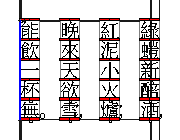
\includegraphics[height = 12\zh]{figure/fig-tc.pdf}\空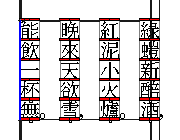
\includegraphics[height = 12\zh]{figure/fig-jp.pdf}
%<en>    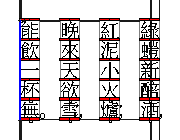
\includegraphics[height = 120pt]{figure/fig-tc.pdf}\quad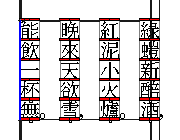
\includegraphics[height = 120pt]{figure/fig-jp.pdf}
%<sc>    \caption{行间标点特性示意图}
%<ja>    \caption{垂直懸垂の機能}
%<en>    \caption{The linegap punctuations feature}
    \label{fig:lgp}
\end{figure}
%<sc>标点悬挂的位置有以下考量,可参照图\ref{fig:lgp}~。若有特殊需求请看第\ref{sec:config}节。优先级由上至下。
%<ja>図\ref{fig:lgp}~に示すように、これらの懸垂句読点の位置は、以下のルールに従って決定されます。カスタマイズについては、サブセクション\ref{sec:config}を参照してください。ルールの優先順位は早い順に高くなります。
%<en>The position of these hanged punctuations is decided according to the following rules as shown in the figure \ref{fig:lgp}. For customizing, see subsection~\ref{sec:config}. The rules which occurs more early have the higher priorities.
\begin{itemize}
%<sc>    \item 三种字体风格统一,位置原则上一致(故,繁中字体也悬挂于右下、而非居中);
%<ja>    \item 3つのフォントのスタイルは統一されています;
%<en>    \item The style of the three fonts are unified;
%<sc>    \item 不同标点中的相同(似)元素位置相同;
%<ja>    \item 異なる句読点における同じ要素の位置は同じであるべきです;
%<en>    \item The position of the similar elements in different punctuations should be the same;
%<sc>    \item 繁中、简中、日文字体标点触字框右边线;
%<ja>    \item 句読点のグリフは漢字の境界に接触するべきです;
%<en>    \item The glyph of the punctuations should touch the \textit{kanji\/}'s boundary;
%<sc>    \item 不同标点符号因形状不同可于字框底线略下沉或上浮;
%<ja>    \item 異なる句読点の位置は、それぞれのグリフの形状、サイズ、デザインに応じて異なる場合があります。
%<en>    \item Different punctuations' position can vary considering their glyphs' shapes, sizes, design respectively.
%<sc>    \item 不同标点符号因大小不同可靠近或远离字框右边线;
%<sc>    \item 三种字体可分别因字符设计的差异而位置略微区别。
\end{itemize}

%<sc>\subsection{用戶配置}
%<ja>\subsection{ユーザー設定}
%<en>\subsection{User Configs}
\label{sec:config}
%<sc>本特性是以三套思源字体为基准设计的。而由于各字体的标点符号位置不可避免会有不同,故在某些特殊情况下会出现错位影响视觉效果的情况。或是单纯对原设定而言更偏好其他设定等原因,本节提供自定义及调整的两种方法。第一种较简单但可移植性较差,而第二种虽繁琐但一劳永逸。
%<ja>この機能はSource Hanフォントシリーズ(思源系列)に設計されています。異なるフォントによって異なる句読点があるため、出力が誤った結果になる可能性があります(オーバーラップ、揃っていないなど)。そのため、懸垂句読点の位置をカスタマイズするための2つの方法が提供されています。
%<en>This feature is designed for the Source Han font series (思源系列). Due to different fonts' different punctuation marks, the output may be wrong (overlap, not aligned, etc). Also you may prefer your own settings. Therefore, two methods of customizing the positions of hanged punctuations is provided here.

%<sc>\subsubsection{修改原程式碼}
%<ja>\subsubsection{パラメータの変更}
%<en>\subsubsection{Changing Parameters}
%<sc>在\textsf{Eva-JFM}中,控制行间标点的分区分别为
%<ja>\texttt{Eva-JFM}では、これらの懸垂句読点の位置に関するパラメータを含むテーブルは以下のようになります
%<en>In \textsf{Eva-JFM}, the tables which contains the parameters for the positions of these hanged punctuations is
\begin{lstlisting}
    [101,2] ==> [1]; [201,2] ==> [2]; [301,2] ==> [3].
\end{lstlisting}
%<sc>只需调整其中\texttt{left}和\texttt{down}键的值即可。其中\texttt{left}为向右移动,\texttt{down}为向下移动。
%<ja>上下のパラメータを調整して、出力を修正してください。
%<en>Kindly modify \texttt{left} (dir right) and \texttt{down} (dir down) until the output is fine.
%<sc>具体可参照终章。
%<ja>また、最後のセクション『実装』も参照してください。
%<en>You can also refer to the last section (\textit{Implementing\/}).

%<sc>\subsubsection{使用外掛符號字體}
%<ja>\subsubsection{追加フォントの使用}
%<en>\subsubsection{Using Extra Font}
%<sc>该方法的原理就是使用特殊的仅包含(标点)符号的字体来替换原有字体中的标点符号,从而稳定其表现。可使用字体煉炉等工具将标点符号从整套字体中提取出来并封装为新字体,也可使用开源符号字体。\段
%<ja>句読点のグリフを抽出して、新しいフォントにパッケージ化し、後で行頭の句読点に使用することが、2番目の解決策です(\textit{Fontforge\/}などのプログラムを使用できます)。また、句読点だけのために別のフォントをロードすることもできますが、CJフォントを{\TeX}のメモリにロードするコストは高くなります。\段
%<en>Extracting the glyphs for punctuation marks and package them into a new font (you can use programs like \textit{fontforge\/}) and use them for hanging punctuations later is the second solution. You can also load another font just for its punctuations (but loading a CJ font into {\TeX}'s memory has an expensive cost).\par
%<sc>将其放入\texttt{TEXMF}并更新\texttt{Ls-R}文件后即可使用\LuaTeX-ja提供的\texttt{AltFont}键进行替换,例元:
%<ja>このフォントをインストールした後、\LuaTeX-jaで提供される\texttt{AltFont}キーを使用して、句読点を置き換えることができます。実際のコードは上記に示されています:
%<en>After installing that font, you can use the \texttt{AltFont} key provided by \LuaTeX-ja to replace the punctuations. The actual code is shown above.
\begin{lstlisting}
    \setmainjfont[
        Language = §\meta{language}§,
        TateFeatures = {
            JFM = eva/{vert, lgp, §\meta{language}§},
            AltFont = {
                {Range = "§\meta{utf-8 code}§, Font = §\meta{symbol font}§}
            }
        }
    ]{§\meta{main font}§}
\end{lstlisting}
%<sc>其中首个\meta{language}可选填\texttt{Japanese}、\texttt{Chinese Traditional}或\texttt{Chinese Simplified},第二个则填语言特性分区的对应\texttt{jp}、\texttt{trad}及\texttt{smpl}特性。\meta{utf-8 code}则为需要替换的标点符号的Unicode编码,如需替换句号(ideographic full stop,\texttt{U+3002})则填\texttt{3002}\footnote{编码可至\url{https://www.unicode.org/charts/unihanrsindex.html}查询。}。
%<ja>最初の\meta{language}オプションには、日本語、繁体字中国語、簡体字中国語のいずれかを入力し、もう一方は対応するJFMの機能のためのものです。 \meta{utf-8 code}は、置き換えたい句読点を「句読点フォント」で選択します\footnote{Unicodeのコードポイントは\url{https://www.unicode.org/charts/unihanrsindex.html}で確認できます。}。最後に、\meta{symbol font}と\meta{main font}オプションは、「句読点フォント」とメインフォントのためのものであることが明らかです。\段
%<en>One of \texttt{Japanese}, \texttt{Chinese} \texttt{Traditional} or \texttt{Chinese} \texttt{Simplified} should be filled in the first \meta{language} option, the other one is for the corresponding JFM features. \meta{utf-8 code} selects the punctuations you'd like to replace with the ``punctuation font''\footnote{You can search \url{https://www.unicode.org/charts/unihanrsindex.html} for their unicodes representations.}.
%<sc>\meta{symbol font}以及\meta{main font}填符号字体名称、正文字体名称即可。\段
%<en>Finally, it's obvious that the \meta{symbol font} and the \meta{main font} options are for the ``punctuation font'' and the main font.\par
%<sc>对于开发者,也建议使用NFSS的
%<ja>開発者は、以下のように NFSS を使用することを推奨します
%<en>It's also recommended for the developers to use the NFSS with
\begin{lstlisting}
    \DeclareAlternateKanjiFont{§\meta{base encoding}§}{§\meta{base family}§}{§\meta{base series}§}{§\meta{base shape}§}{§\meta{alt encoding}§}{§\meta{alt family}§}{§\meta{alt series}§}{§\meta{alt shape}§}{§\meta{range}§}
\end{lstlisting}
%<sc>进行替换。其中\meta{base}为正文字体,\meta{alt}则为替换符号字体。\段
%<ja>オプション\meta{base}と\meta{alt}は、メインフォントと「句読点フォント」のためのものです。\段
%<en>Option \meta{base} and \meta{alt} stands for main font and ``punctuation font''.\par
%<sc>具体语法及示例可看\LuaTeX-ja文档\cite{luatexja-doc}。
%<ja>詳しい構文や使用方法、例については、\LuaTeX-jaのドキュメント\cite{luatexja-doc}を参照してください。
%<en>Refer to the \LuaTeX-ja document~\cite{luatexja-doc} for more detailed syntax and usage as well as some examples.

%<sc>\section{启發}
%<ja>\section{インスピレーション}
%<en>\section{Inspiration}
%<sc>\textsf{Eva-JFM}的内部分组受\texttt{min10.tfm}~\cite{min10}的启发,支持的\texttt{priority}特性则取自阿部紀行氏的\texttt{jlreq.lua}~\cite{ltxjlreq}文件。其余可见参考文献。\段
%<ja>\textsf{Eva-JFM}の内部グループ化は、\texttt{min10.tfm}~\cite{min10}に触発されています。また、優先度の特徴のデータは、阿部紀行氏の\texttt{jlreq.lua}~\cite{ltxjlreq}から一部引用しています。\段
%<en>\textsf{Eva-JFM}'s internal grouping is inspired by \texttt{min10.tfm}~\cite{min10}, while its \texttt{priority} feature's data partly comes from Noriyuki Abe's \texttt{jlreq.lua}~\cite{ltxjlreq}.\par
%<sc>本JFM的名字来源于庵野秀明的『新世紀エヴァンゲリオン』。
%<ja>このJFMの名前は、庵野秀明氏のアニメーション『新世紀エヴァンゲリオン』。
%<en>This JFM's name comes from the animation \textit{Neon Genesis Evangelion\/} by Hideaki Anno.

\begin{thebibliography}{9}
    \addcontentsline{toc}{section}{\refname}
    \bibitem{jlreq} W3C Japanese Layout Task Force~(ed). \newblock Requirements for Japanese Text Layout (W3C Working Group Note), 2022, 2023. \newblock \url{https://www.w3.org/TR/jlreq/}.
    \bibitem{luatexja-doc} \LuaTeX-jaプロジェクトチーム. \newblock \LuaTeX-jaパッケージ, 2022, 2023.
    \bibitem{unicode} The Unicode Consortium. \newblock The Unicode Standard Version 15.0 - Core Specification, 2022.
    \bibitem{tex-by-topic} Victor Eijkhout. \newblock \TeX{} by Topic, A \TeX nician's Reference, Addison-Wesley, 1992.
    \bibitem{min10} 乙部厳己. \newblock min10フォントについて. \newblock \url{http://argent.shinshu-u.ac.jp/~otobe/tex/files/min10.pdf}.
    \bibitem{ltxjlreq} 阿部紀行. \newblock Jlreq Document Class, 2022. \newblock \url{https://github.com/abenori/jlreq}.
    \bibitem{evang} 庵野秀明. \newblock 新世紀エヴァンゲリオン.
\end{thebibliography}

%<ignore>\section*{程式碼}
%<ignore>\section*{実装}
%<ignore>\section*{Implementation}
%<ignore>以下为\texttt{jfm-eva.lua}文件内容,供参考。%及二次开发等。
%<ignore>The above is the implementation of this font metric. Can be used for reference.
%<ignore>\lstinputlisting{jfm-eva.lua}

\end{document}
